\chapter{基于FPGA的循环神经网络加速器实验分析}
上一章详细介绍了循环循环神经网络加速系统的设计,包括系统总体架构设计,功能划分,软硬件设计及其具体实现,系统的各个组成部分分工协同,
组成了可动态调节精度和速度的循环神经网络加速系统。本章将从实验的角度对系统设计的各项目标进行检测,实验的内容包括验证系统的基本功能是否正常,系统的资源消耗是否合理,
以及系统的运行速度和功耗能否满足系统设计要求。最后,在完成上述实验的基础上,本章将对系统的优势进一步说明。
\section{实验方案设计}
\subsection{实验环境}
硬件平台:如图~\ref{fig_board},本章实验采用Nexys4 DDR开发板作为本文系统的硬件平台。Nexys4 DDR开发板内部集成了Artix-7系列的FPGA芯片,型号为XCA100T-1CSG324C。
该芯片采用28nm的高效能/低功耗(HPL)制程技术,能够在极低功耗的前提下突破许多性能极限,广泛应用于低功耗的场景。此外,开发板还配置了容量为128MB的DDR存储器,
能满足多数应用的存储需求,Microblaze软处理器等技术支持也使得设计人员可以基于FPGA快速搭建SOC系统。低功耗,高能效,便捷性是本文选取Nexys4 DDR作为硬件平台的
重要原因,同时由于A7系列FPGA芯片的资源相对有限,而一般情况下,循环神经网络加速器需要消耗大量的资源,因此解决这一组矛盾也符合本文系统设计的初衷。

开发工具:本文使用Xilinx公司的FPGA开发套件,包括Vitis HLS, Vivado以及Vitis SDK。这些开发工具能提供从软件设计,硬件实现到软硬件系统的集成等系统
设计的全部任务流程。

神经网络训练:循环神经网络结构的搭建采用TensorFlow (Tensorflow Addons, TFA) 框架下的ESN网络模型,网络的训练方法是线性回归。
在完成网络参数的训练后需要将参数提取出来以进行后续的压缩过程。压缩算法的验证基于NumPy设计实现,简化网络的功能验证也在此环境下进行。最后保存训练好的
原始网络模型参数以及必要的压缩算法所需的数据。
\begin{figure}
	\centering
	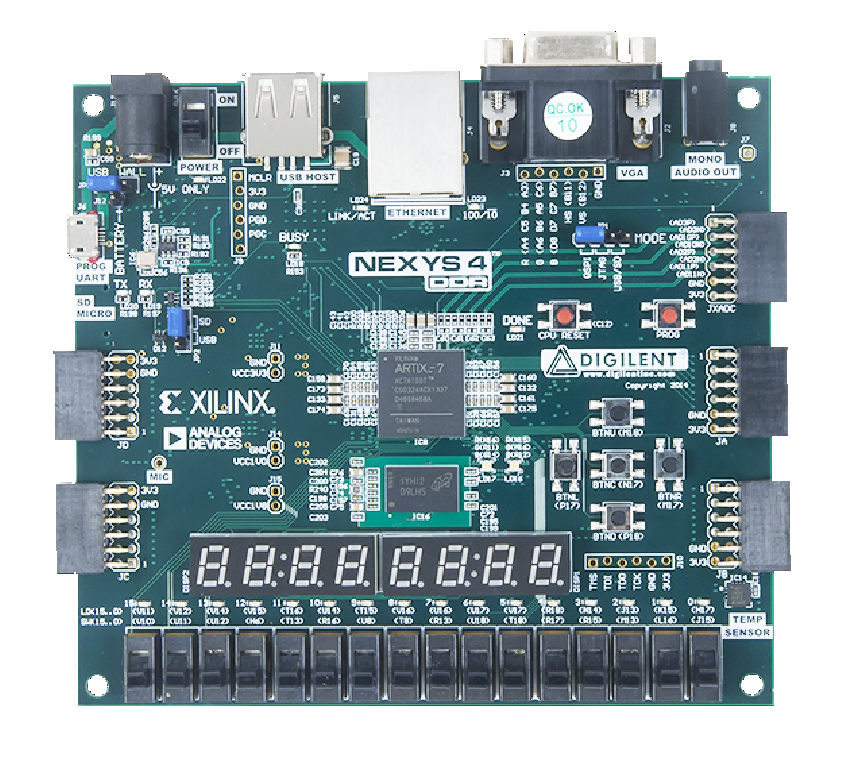
\includegraphics[width=0.6\columnwidth]{FPGA_board.eps}
	\caption{本文系统实现所使用的Nexy4 DDR 开发板,集成了A7系列的FPFA芯片和DDR芯片}
	\label{fig_board}
\end{figure}
\subsection{实验内容}
在算法分析及系统架构设计章节,本文详细的论述了系统设计的细节并展示了其所具有的潜在优势,例如从功能的角度,本文的系统设计能满足应用场景对
模型预测速度和精度动态调节的需求,能在资源有限的设备上独立运行,能实现和环境的数据交互等。从硬件实现的角度,本文所设计的硬件加速器具有高度复用的模块,极大的降低了
硬件资源的消耗。针对以上优势,本章设计了以下实验内容进行证明:

1.系统运行效果的实验:根据任务的难易程度以及任务的输入输出特点,本文选取了不同的测试集进行系统功能的测试。测试集包括单输入单输出系统:
NARMA10,NARMA30和复杂二阶问题,多输入多输出系统:两入两出非线性系统。系统在运行这些任务时需要测试的功能
包括更改简化网络的模型尺寸,状态采样以及原始网络模型的压缩等。系统功能的正常是系统设计的首要目标,也是系统功能优势的实际体现。

2.加速器性能实验:本文对循环神经网络前向传播过程设计了专用硬件架构以实现加速的目的,加速器性能的主要指标有资源消耗,数据吞吐率(速度)以及功耗。
本实验将对这些指标分别进行测量,并将其与硬件设计相联系,说明本文加速器设计的特点和优势。

\section{系统运行效果}
实验设定:系统运行不同的任务,在连续输入的过程中切换模型尺寸,并以该尺寸的简化网络模型进行前向传播。简化网络模型的权重参数的生成有两种方法:
基于状态采样的模型生成方法和基于预置投影矩阵的模型生成方法,这两种方法分别对应系统的两种应用环境:异常状态环境和普通环境。在普通环境下,
网络的实际状态与预存的状态空间偏离较小,通过增大投影空间的方法可以实现状态的“准确”近似;在异常状态环境下,由于特征空间是有限的,无法囊括
所有的状态,少量实际存在的状态将在压缩的过程中被合理的丢失,然而在系统实际运行过程中难免会遇到这种情况,因此系统需要和实际环境进行数据交换,
通过采样的方法生成网络的权重参数。

本实验测量两种压缩模型生成方法下的模型预测效果。连续输入的序列长度为1000个,在完成该段序列的预测后,系统将会切换简化网络的模型尺寸并进行下一段序列的预测。
本实验依次设定简化网络模型阶数为10,20,30,40,60,80。实际上,在硬件支持的简化模型最大尺寸以下,简化网络模型尺寸可以设定为任意整数值。
%说明压缩算法能在边缘设备实现,加速器可以运行不同尺寸的网络模型。

\subsection{复杂二阶问题}
复杂二阶问题建模了一个二阶动态系统,该系统的数据依赖呈现指数相关的关系,即输入序列中的关键信息会被指数放大,而无关特征则会被迅速遗忘。
其数学表达为
\begin{equation}
	y(t+1) = \frac{y(t)y(t-1)(y(t)+0.25)}{1+y^2(t)+y^2(t-1)} + u(t)
\end{equation}
其中\(u(t)\)是在区间\([0,0.5]\)上生成的均匀分布的随机数。
\begin{center}
\begin{table}
	\caption{在二阶问题上简化网络不同模型尺寸的预测精度}
	\renewcommand\arraystretch{1.2}
	\setlength{\tabcolsep}{12pt}
	\begin{tabular}{ccccccc}
	\toprule
		 							&	10		&	20		&	30		&	40		&	60		&	80		\\	\midrule
	Sample M.\(\times 10^{-4}\)	&	2.99	&	2.58	&	2.46	&	0.81	&	0.25	&	0.11	 \\	\hline
	PreStore M.\(\times 10^{-4}\)&	36.3	&	18.5	&	9.9		&	6.9		&	1.7		&	0.53	\\	
	\bottomrule
	\label{tab:second}
	\end{tabular}
\end{table}
\vspace{-3em}
\end{center}



系统在二阶问题任务上的运行效果如图~\ref{fig:second} 所示,可以看出不同尺寸的简化网络模型的预测值均能较好的还原系统的真实输出。这里系统的真实输出可以
用原始网络模型的预测值进行准确的代替,一方面是因为原始网络模型的输出和系统真实输出误差较小,另一方面是因为在实际情况下测量系统的真实输出一般具有
滞后性,并且可能存在测量成本大等无法获得真实数据等情况。图中左侧是基于采样方法生成的简化网络模型,由上至下,模型的阶数依次增加。其中10阶的简化网络模型
预测效果和系统真实输出存在明显的偏差,随着简化网络模型尺寸的增大,模型的预测逐渐贴合系统的真实输出。图中右侧为基于预置投影矩阵方法生成的简化网络模型,
图中显示,该方法生成的简化网络模型在不同的模型尺寸下均拥有较小的误差。这说明小尺寸网络模型依然能胜任二阶问题的模型预测,网络精度的调节可以在
小尺寸网络的基础上进行小幅度改变即可。

表~\ref{tab:second} 展示了两种模型生成方法下不同尺寸简化网络模型的预测精度,误差的数值随着模型尺寸的增加而降低,其中采样方法生成的简化网络误差
降低更加明显。这说明了状态空间越大,状态信息越丰富,其所生成的投影空间和真实的特征空间偏差越小。由于预置的投影矩阵的生成往往采样了
足够多的状态数据,因此即使在相同的模型尺寸下,通过预存投影矩阵的方法生成的模型预测精度高于现场采样生成模型的精度。但是这并不能说明采样
方法不是系统所需要的功能。相反,由于该方法不依赖于任何先验信息,可以和环境交互数据,这使得即使系统处在异常环境中,也具有较高的预测能力。
两种方法互为补充,共同实现系统高精度预测的功能。
\begin{figure}
	\centering
	\subfloat[]
	{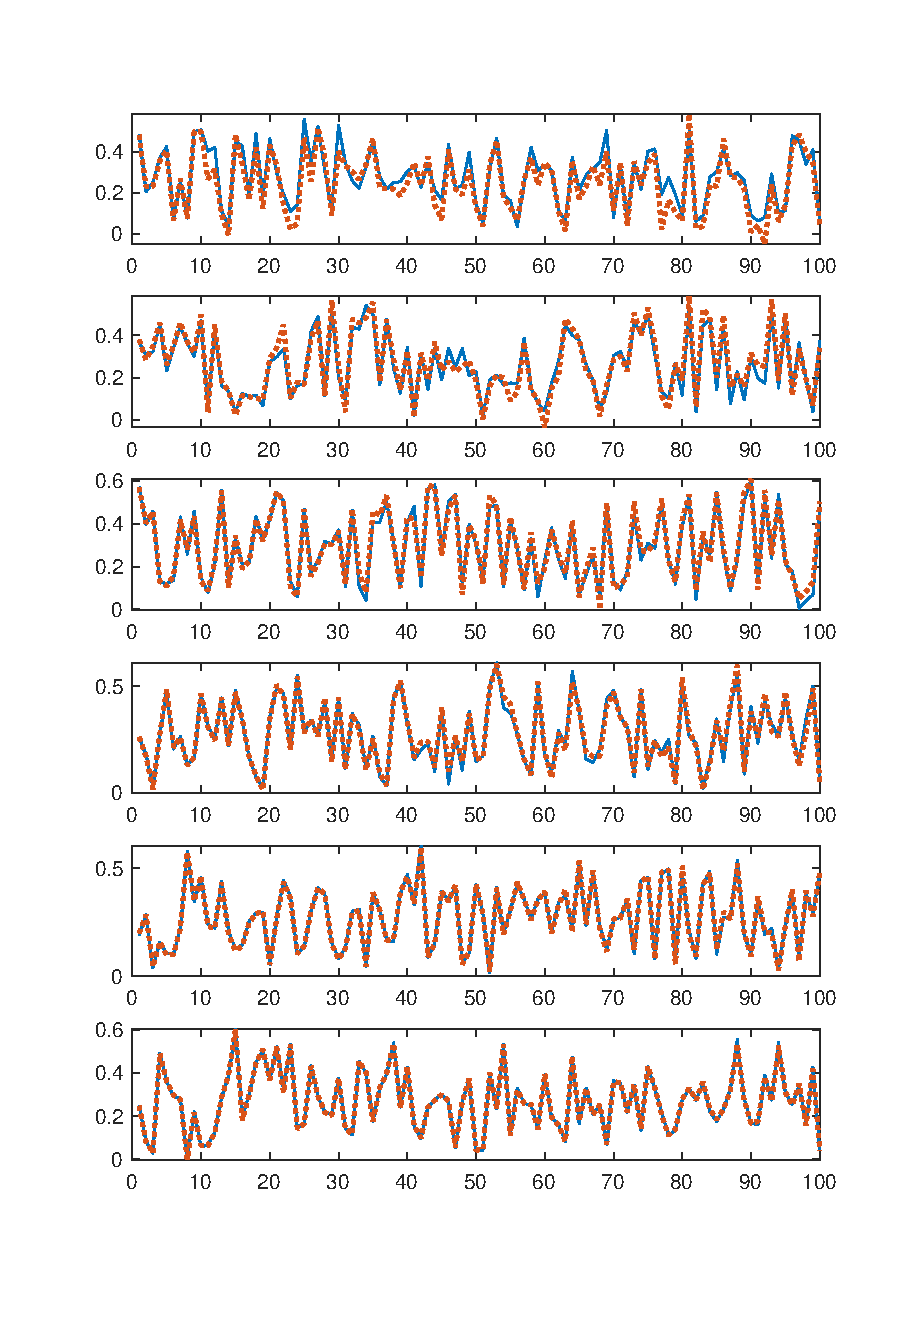
\includegraphics[width=0.5\columnwidth]{exp/fig_second_gen.eps}\label{fig:second_gen}}
	\subfloat[]
	{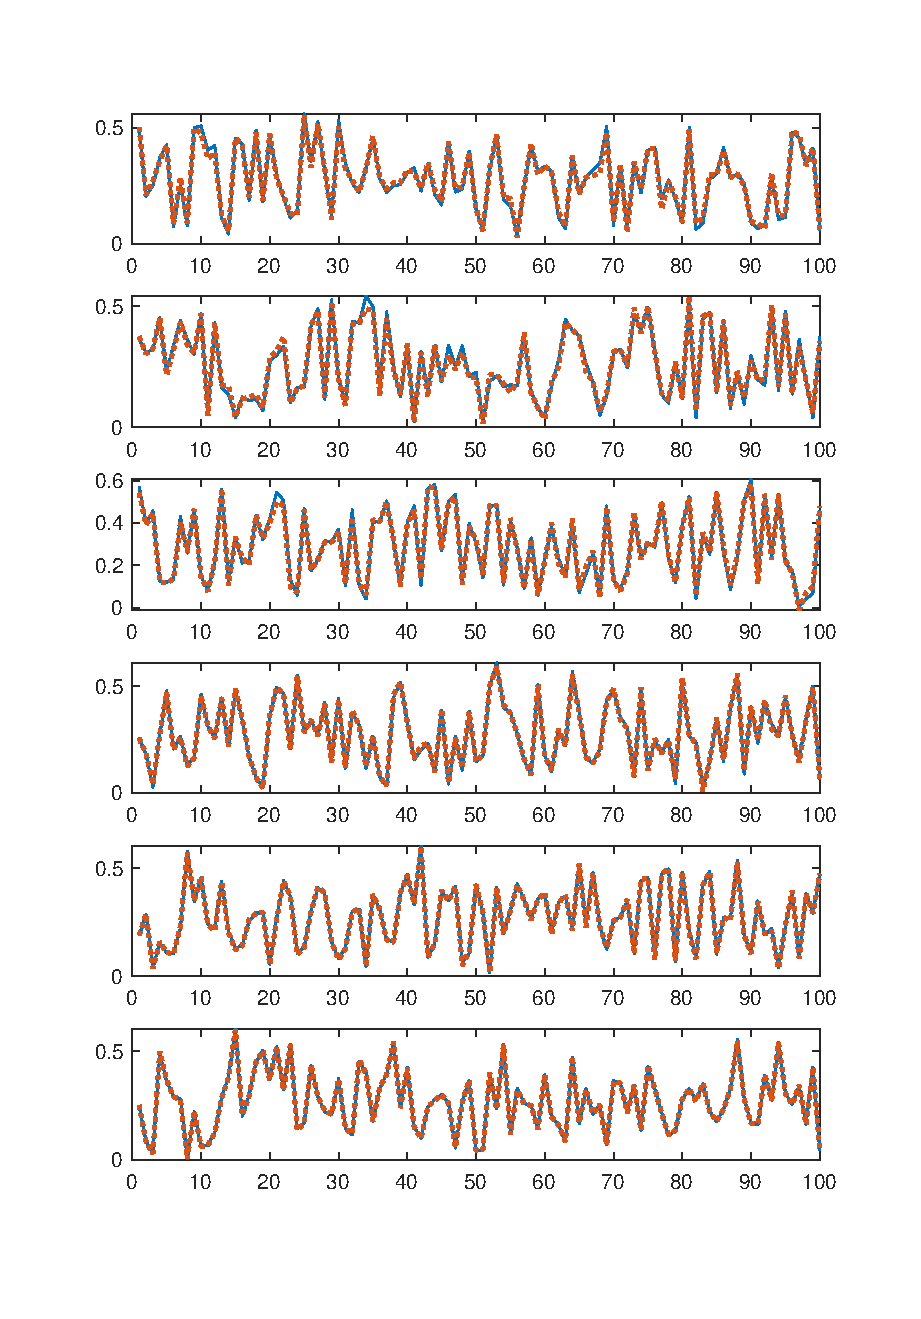
\includegraphics[width=0.5\columnwidth]{exp/fig_second_pre.eps}\label{fig:second_pre}}
	\caption{在复杂二阶问题上的系统运行效果,实线表示原始网络的预测值,点线表示简化网络的预测值。
		图a是使用采样方法的系统预测效果,图b是使用预存投影矩阵方法的系统预测效果。图a和图b自上而下的子图中的简化网络阶数分别为10,20,30,40,60,80。}
	\label{fig:second}
\end{figure}


本文所设计的系统在二阶问题的任务的解决上,系统能够发现应用的实现难度较低进而主动降低简化网络模型的尺寸,并以较小的模型尺寸进行前向传播,
实现了高速的模型预测。相较于其他神经网络加速方法的一次性设计,本文的系统对任务的难易程度具有一定的感知能力。

\subsection{两个NARMA系统}

NARMA(Nonlinear Auto Regressive Moving Average)定义了具有长期依赖关系的动态系统,即很久以前的输入对系统当前的输出仍存在影响。循环神经
网络尽管能够学习这些长程依赖关系,但是依然存在一些难以解决的问题,例如对处理此类任务的循环神经网络进行压缩,压缩过程中损失的信息可能导致
网络失去长期记忆而功能瘫痪。本文选取该任务进行系统运行效果测试,以验证系统在长期记忆的复杂任务中依然具有适用性。NARMA10系统的数学表达为
\begin{equation}
	y(t) = 0.3y(t-1) + 0.05y(t-1)\sum_{i=1}^{10}y(t-i) + 1.5u(t-9)u(t) + 0.1
\label{eq:narma10}
\end{equation}
NARMA30系统的数学表达为
\begin{equation}
	y(t) = 0.2y(t-1) + 0.04y(t-1)\sum_{i=1}^{30}y(t-i) + 1.5u(t-29)u(t) + 0.001
\label{eq:narma30}
\end{equation}
由式~(\ref{eq:narma10}) 和~(\ref{eq:narma30}) 可知,这两个系统的最大延迟时间步长分别为10和30。
\begin{figure}
	\centering
	\subfloat[]
	{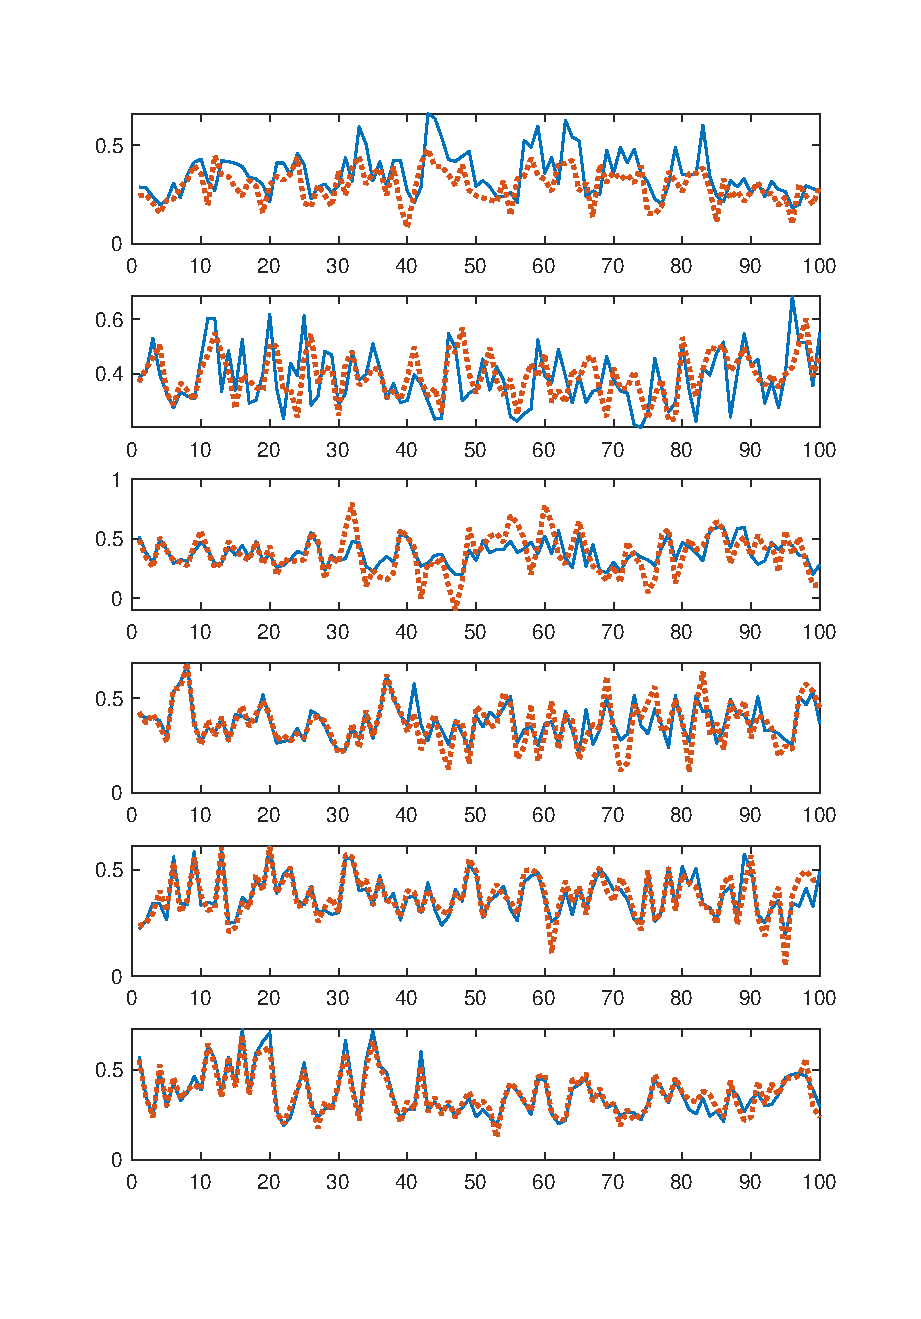
\includegraphics[width=0.5\columnwidth]{exp/fig_narma10_gen.eps}\label{fig:narma10_gen}}
	\subfloat[]
	{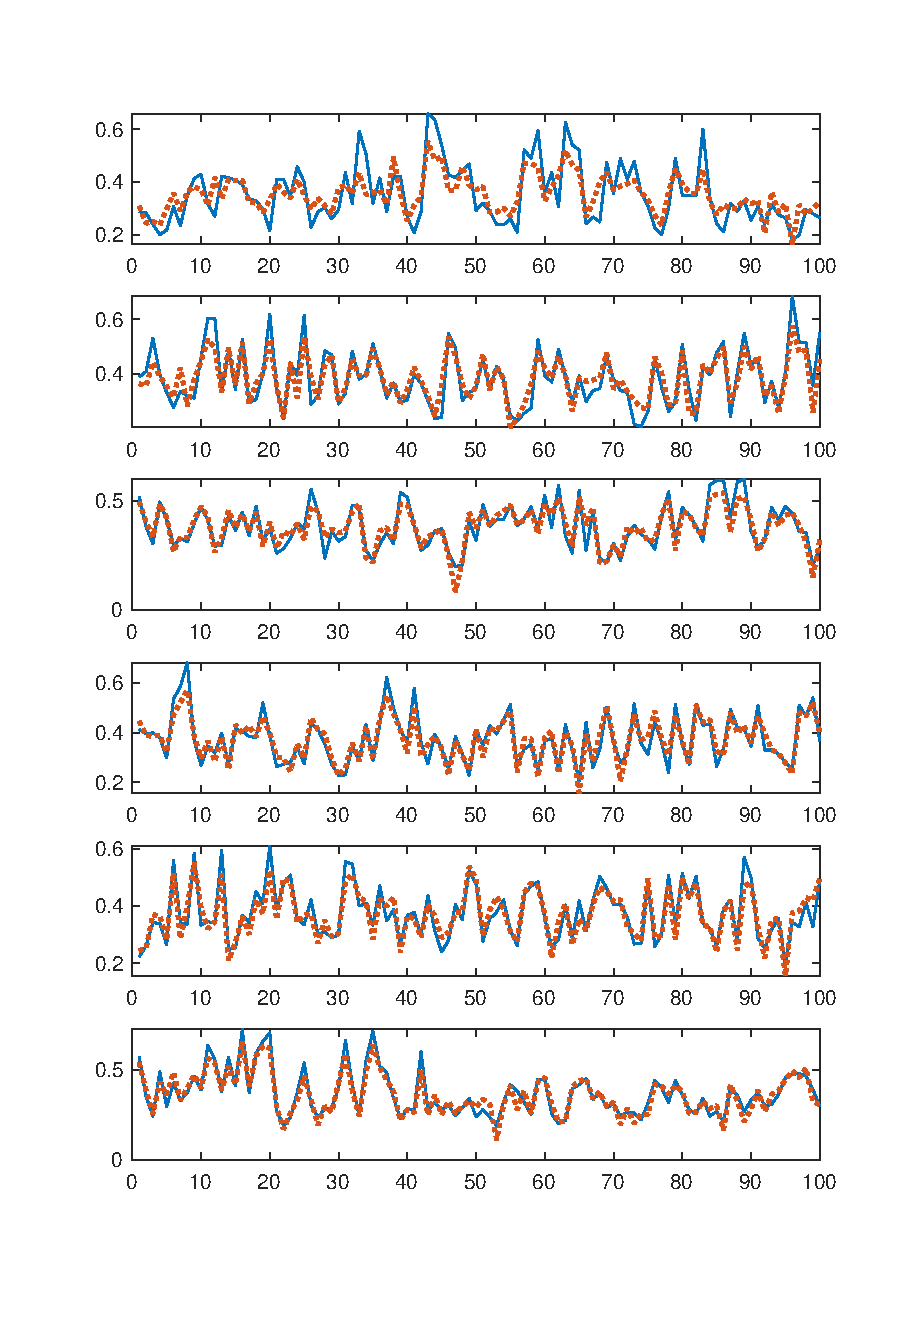
\includegraphics[width=0.5\columnwidth]{exp/fig_narma10_pre.eps}\label{fig:narma10_pre}}

	\caption{在NARMA10任务上的系统运行效果,实线表示原始网络的预测值,点线表示简化网络的预测值。
		图a是使用采样方法的系统预测效果,图b是使用预存投影矩阵方法的系统预测效果。图a和图b自上而下的子图中的简化网络阶数分别为10,20,30,40,60,80。}
	\label{fig:narma10}
\end{figure}

\begin{center}
\begin{table}
	\caption{在NARMA10任务上不同尺寸简化网络模型的预测精度}
	\renewcommand\arraystretch{1.2}
	\setlength{\tabcolsep}{12pt}
	\begin{tabular}{ccccccc}
	\toprule
		 							&	10		&	20		&	30		&	40		&	60		&	80		\\	\midrule
	Sample M.\(\times 10^{-3}\)		&	4.2		&	1.7		&	1.6		&	1.5		&	1.3		&	1.2	 \\	\hline
	PreStore M.\(\times 10^{-3}\)	&	13.4	&	4.3		&	9.4		&	5.1		&	2.6		&	1.6	\\	
	\bottomrule
	\label{tab:narma10}
	\end{tabular}
\end{table}
\vspace{-3em}
\end{center}


图~\ref{fig:narma10} 所示为系统在NARMA10任务上的运行效果。由于任务的复杂度变高,小尺寸的简化网络模型在该任务上预测误差较大,其只能捕捉任务的变化趋势,
而对任务的具体细节则无法准确预测。当模型尺寸在40阶及其以上时,两种方法所生成的简化网络模型均能较好的预测任务的真实输出。对比两种模型生成方法下的网络
预测效果,当网络尺寸较大时,两种方法能获得相似的预测精度,在某段序列的预测上,采样方法甚至能获得更高的精度;当网络尺寸较小时,由于采样的的状态数量少,投影空间
包含的特征信息少,因此预测效果较基于预置投影矩阵的方法误差更大。
\begin{figure}[htb]
	\centering
	\subfloat[]
	{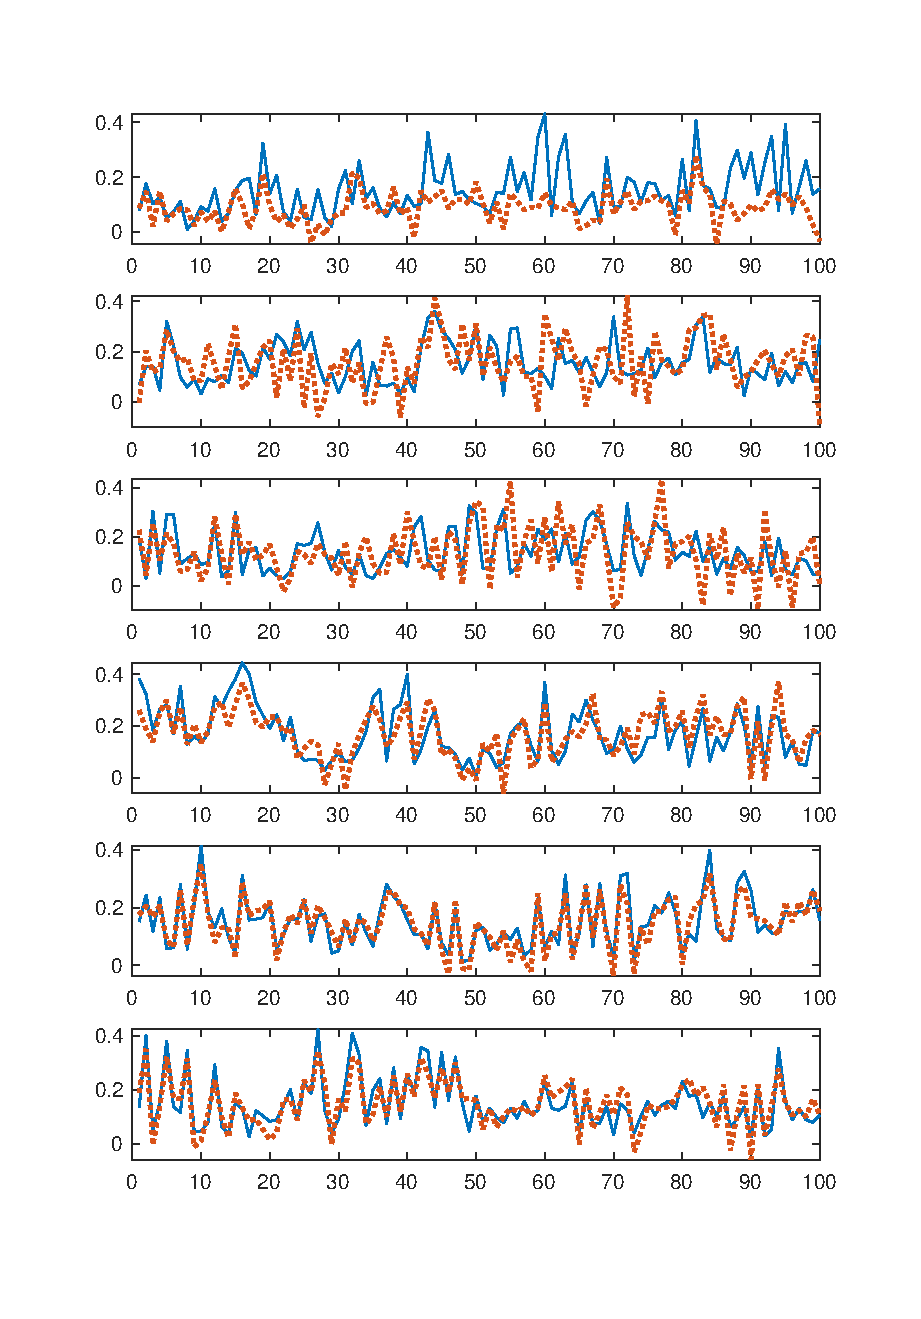
\includegraphics[width=0.5\columnwidth]{exp/fig_narma30_gen.eps}\label{fig:narma30_gen}}
	\subfloat[]
	{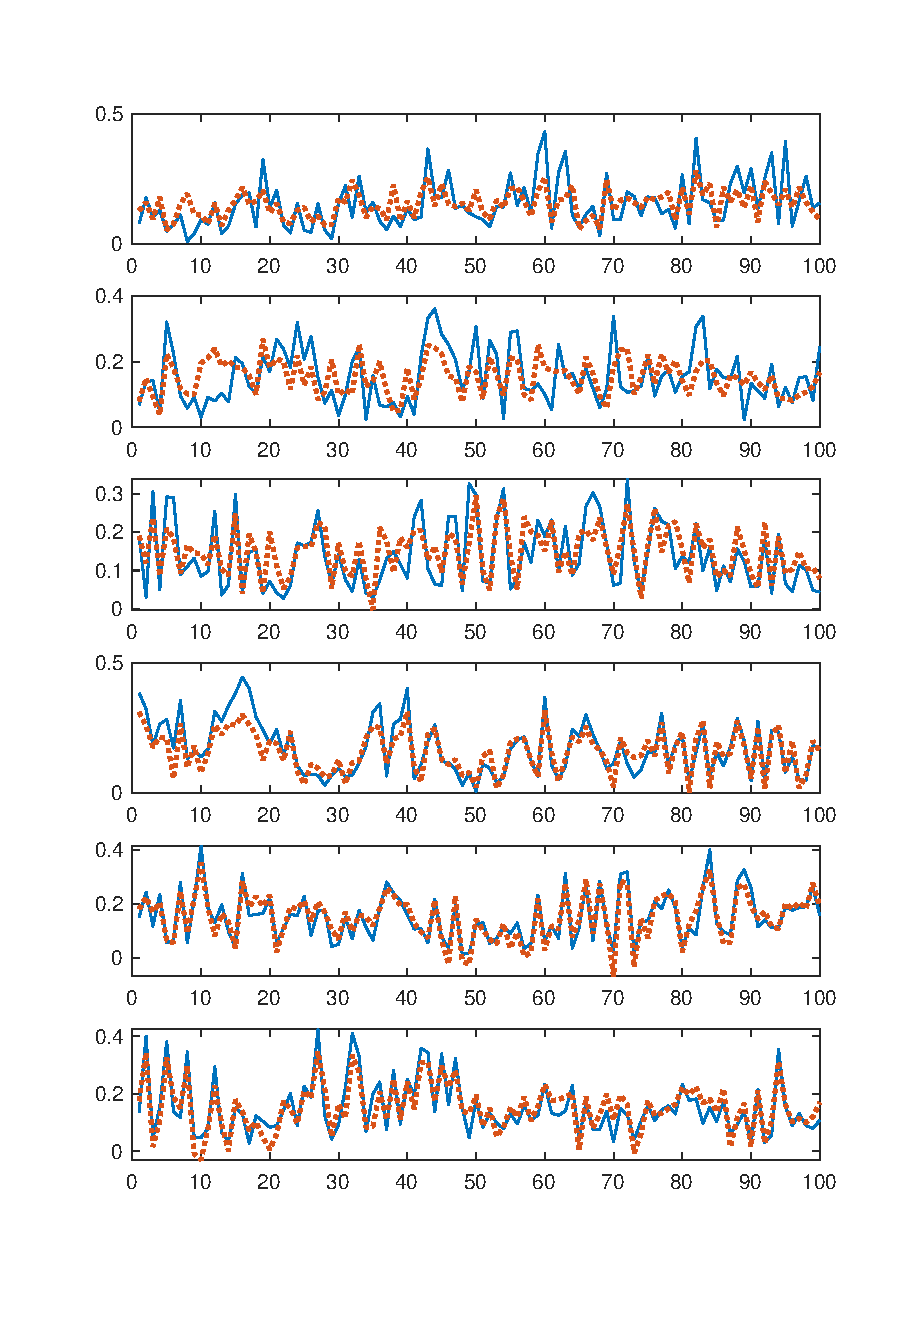
\includegraphics[width=0.5\columnwidth]{exp/fig_narma30_pre.eps}\label{fig:narma30_pre}}
	\caption{在NARMA30任务上的系统运行效果,实线表示原始网络的预测值,点线表示简化网络的预测值。
		图a是使用采样方法的系统预测效果,图b是使用预存投影矩阵方法的系统预测效果。图a和图b自上而下的子图中的简化网络阶数分别为10,20,30,40,60,80。}
	\label{fig:narma30}
\end{figure}
\begin{center}
\begin{table}
	\caption{在NARMA30任务上不同尺寸简化网络模型的预测精度}
	\renewcommand\arraystretch{1.2}
	\setlength{\tabcolsep}{12pt}
	\begin{tabular}{ccccccc}
	\toprule
		 							&	10		&	20		&	30		&	40		&	60		&	80		\\	\midrule
	Sample M.\(\times 10^{-3}\)		&	5.1		&	5.0		&	3.3		&	1.7		&	1.4		&	1.3	 \\	\hline
	PreStore M.\(\times 10^{-3}\)	&	10.1	&	26.6		&	17.7		&	5.3		&	2.6		&	2.4	\\	
	\bottomrule
	\label{tab:narma30}
	\end{tabular}
\end{table}
\vspace{-4em}
\end{center}


图~\ref{fig:narma30} 所示为系统在NARMA30上的运行效果,相比于NARMA10,任务更加复杂。因此当简化网络模型的尺寸在60阶及其以上时,系统的预测才能较好的贴合
任务的真实输出,而在小网络尺寸例如10阶的简化网络模型,系统甚至难以预测任务的变化趋势。

系统在两个NARMA任务上的预测精分别如表~\ref{tab:narma10} 和表~\ref{tab:narma30} 所示。随着简化网络模型尺寸的增大,系统的误差也在不断降低。其中基于预存投影矩阵的简化网络
生成方法的精度变化不明显,而采样方法的误差会大幅降低。在以上两个基本规律下,存在个别反常现象,例如在NARMA30任务上10阶的模型的预测精度较低。这是因为系统对
环境数据进行采样时,样本点之间的相关性较弱,这使得样本集的信息量增加,对系统真实行为的相似度越高。这也说明,样本点对系统精度存在较大的影响,而现场采样
正是对预存采样信息的有效补充,因此采样方法也是保证系统独立性的重要环节。

本文所设计的系统在对复杂任务的处理上,不同模型尺寸的预测效果表现出较大的差异,系统可利用该特性实现系统唤醒以及精细化处理等功能。当任务在实际环境中
的重要程度不高时,系统运行小尺寸的网络模型,仅保留对任务的基本处理能力;当环境需要依赖该任务的处理结果时,系统可以切换到较高的模型尺寸进行精细化的处理。

\subsection{两输入两输出非线性系统}
从动态系统的输入输出数量的角度,前面的实验都是在单输入单输出任务上进行测试。为验证本文所设计的系统在多输入多输出的任务上具有适用性,本小节
的实验选取了两输入两输出非线性系统作为测试任务,其数学表达为
\begin{equation}
	\begin{split}
		&x_1(t) = 0.5x_1^{2/3}(t-1) + 0.3x_2(t-1)x_3(t-1) + 0.2u_1(t)	\\
		&x_2(t) = 0.5x_2^{2/3}(t-1) + 0.3x_2(t-1)x_1(t-1) + 0.2u_1(t)	\\
		&x_3(t) = 0.5x_3^{2/3}(t-1) + 0.3x_1(t-1)x_3(t-1) + 0.2u_2(t)	\\
		&y_1(t) = 0.7(x_1(t) + x_2(t))									\\
		&y_2(t) = 1.5x_1^{2}(t)	
	\end{split}
\label{eq:2In2Out}
\end{equation}
式中\(x_1,x_2,x_3\)是动态系统的三个状态,\(u_1,u_2\)是两个输入,输入的取值是\([0,0.5]\)区间内的均匀分布随机数,\(y_1,y_2\)是两个输出。

系统在两输入两输出任务上的运行效果如图~\ref{fig:2In2Out} 所示。其中误差最明显的系统运行效果来自于使用采样方法生成的10阶简化网络模型,
系统的预测与任务的真实输出存在一个固定的偏差值,这主要是由于采样的状态信息不够丰富。为了提高压缩过程的实现速度,本文设置采样的状态数量
和需要生成的简化网络模型阶数相同。随着简化网络模型尺寸的增加,采样方法生成的简化网络的模型将会消除这种偏差,并能以较高的精度还原任务的真实
输出。这说明采样方法存在缺陷,该方法生成的模型只能在采样的时间点附近拥有较高的精度,而在远离采样点的时刻则会精度较低。因此采样方法适用
于异常状态环境,系统能使用此方法在一段时间内获得精度方面的显著增益。但普通环境由于需要长时有效,因此一般选用预存投影矩阵的方法
生成简化网络模型。

表~\ref{tab:2In2Out} 展示了系统在两输入两输出任务上的模型预测精度。除过使用采样方法生成10阶简化网络模型的预测误差较大以外,其他的网络模型
均能实现较高的精度。实际上,系统在该任务上的最差的预测仍然能捕获任务的动态变化特性。

\begin{figure}
	\centering
	\subfloat[]
	{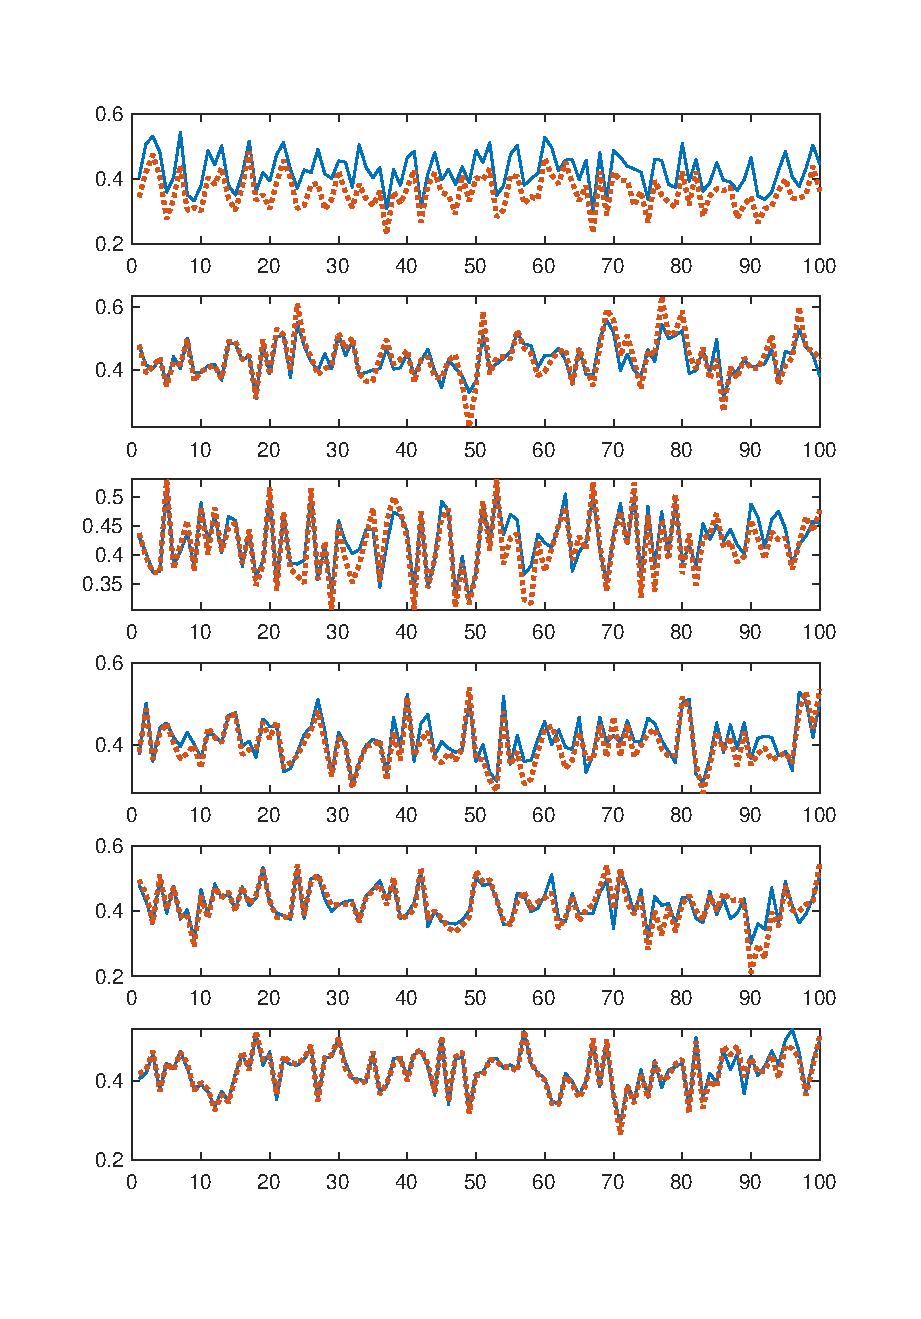
\includegraphics[width=0.5\columnwidth]{exp/fig_2In2Out_gen.eps}\label{fig:2In2Out_gen}}
	\subfloat[]
	{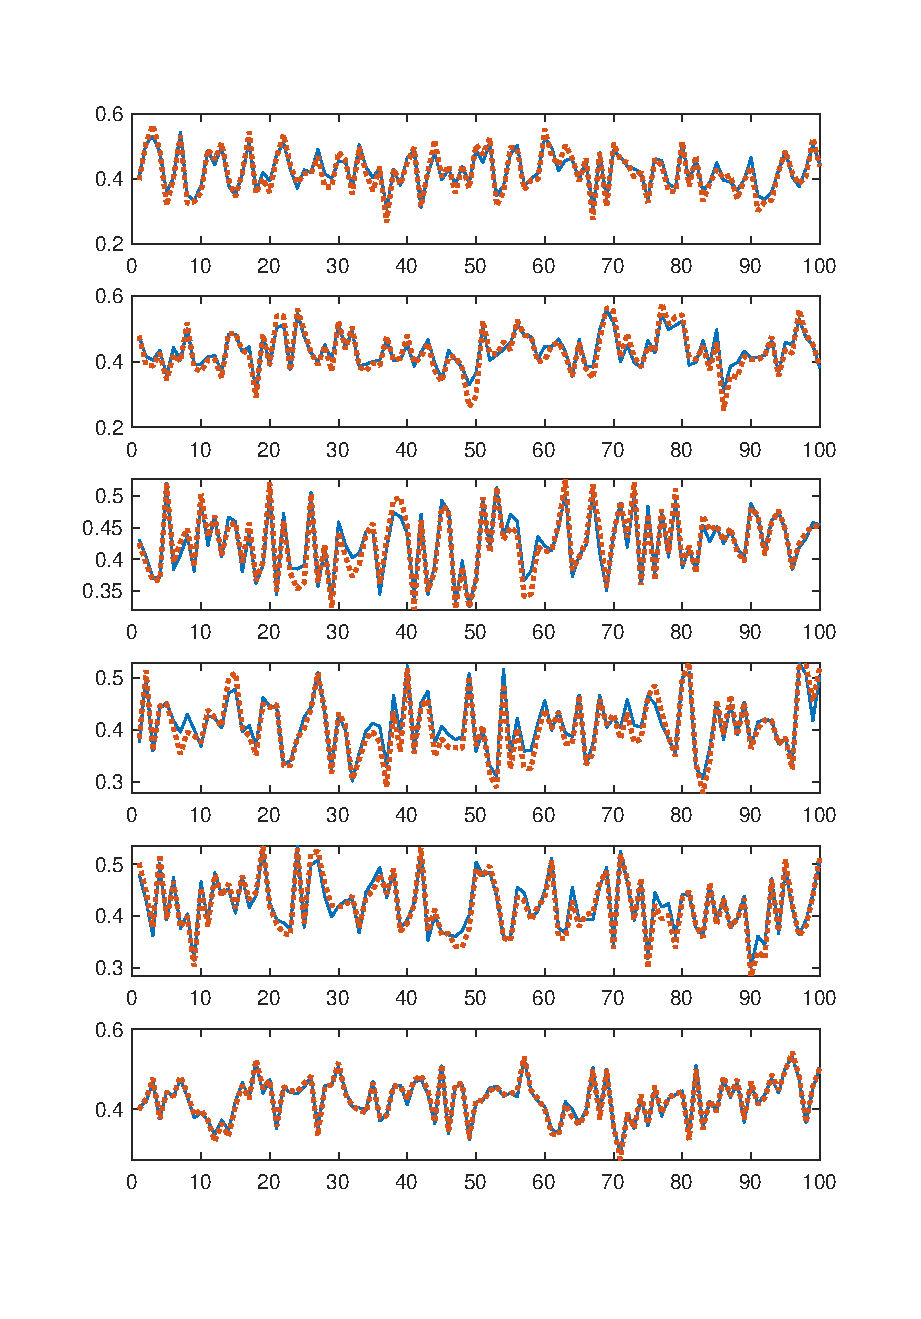
\includegraphics[width=0.5\columnwidth]{exp/fig_2In2Out_pre.eps}\label{fig:2In2Out_pre}}
	\caption{在两输入两输出非线性问题上的系统运行效果,实线表示原始网络的预测值,点线表示简化网络的预测值。
		图a是使用采样方法的系统预测效果,图b是使用预存投影矩阵方法的系统预测效果。图a和图b自上而下的子图中的简化网络阶数分别为10,20,30,40,60,80。}
	\label{fig:2In2Out}
\end{figure}
\begin{center}
\begin{table}
	\caption{在两输入两输出非线性问题上简化网络不同模型尺寸的预测精度}
	\renewcommand\arraystretch{1.2}
	\setlength{\tabcolsep}{12pt}
	\begin{tabular}{ccccccc}
	\toprule
		 									&	10		&	20		&	30		&	40		&	60		&	80		\\	\midrule
	Sample M.~(\(\times 10^{-4}\))			&	4.8		&	3.1		&	2.2		&	2.1		&	1.6		&	0.6	 \\	\hline
	PreStore M.~(\(\times 10^{-4}\))	&	67.4	&	6.7		&	8.1		&	7.2		&	6.5		&	4.7	\\	
	\bottomrule
	\label{tab:2In2Out}
	\end{tabular}
\end{table}
\vspace{-3em}
\end{center}



本文所设计的系统能够胜任多输入多输出任务,并且配备了完善的解决方案以适应不同的运行环境。当系统运行在普通环境时,简化网络模型的生成一般
选用预存投影矩阵的方法;当系统运行在异常状态环境时,通过采样的方法获取异常状态信息,系统能在异常环境中获得较高的精度增益。%改进空间:将异常状态合并到投影矩阵中。
\\

经过以上不同类型任务的测试,本文所设计的系统均表现出良好的兼容性。首先系统的功能基本正常, 系统在运行过程中能切换简化网络模型的尺寸并以设定的尺寸进行
前向传播,网络的权重参数可以通过状态采样方法和预存投影矩阵的方法生成。在以上前向传播和网络压缩功能的相互配合下,系统表现出更高级的功能特性。
系统对任务,环境和用户需求存在一定的感知能力并能做出相应调整,例如根据任务的难易程度和精度要求,系统能动态调节简化网络的模型尺寸;当系统运行在
异常状态环境下,系统使用状态采样的方法以获取一段时间内的较高精度增益。此外,系统还表现出独立性与功能的完整性,系统基于FPGA平台实现,不需要额外的算力
和数据支持。综上所述,本文基于FPGA实现的系统满足系统设计目标,并表现出符合预期的优势。
%采样方法 样本覆盖的位置精度高

%在该类应用中的优势

%最后对系统运行效果进行总结


\section{加速器性能实验}

加速器负责实现网络的前向传播过程,而该过程是系统最主要的功能,因此测量加速器的性能是必要的,其在一定程度上也能反映出系统的整体性能。本小节将从
速度,资源消耗以及功耗等方面对性能进行分析与测量。由于加速器的性能仅决定于加速器的硬件设计与实现,而与具体的任务关联度较小,所以
本实验的吞吐率(速度)和功耗数据都是系统运行NARMA10任务时采集的。
\subsection{吞吐率}
吞吐率是最直观的衡量系统运行速度和延迟的综合性指标,其含义是单位时间处理的系统输入的数量。影响吞吐率的因素主要包括系统频率,运算量,访存延迟等,
是系统各个要素综合作用的结果。本文所设计的加速器结构能够运行不同结构的网络模型:包括原始网络模型和简化网络模型,能够更改网络模型的尺寸:本文主要是指
简化网络的尺寸。以上各种系统运行模式存在不同的计算量和存储量,因此也存在吞吐率的差异。差异化的吞吐率即代表着系统推理的速度可以调节,这能满足用户
和环境对速度的弹性化需求,也是本文系统设计的主要特点之一。

本实验分别测量不同网络结构和不同模型尺寸条件下任务的完成时间作为计算吞吐率的依据,任务的序列长度为10000个,加速器的运行频率是100MHz,时间的计量
采用串口输出计时的方式实现。实际上,吞吐率和任务的完成时间呈倒数关系,两者表示的是同一事物,本文更形象且方便的描述其为速度。

表~\ref{tab:time} 所示为加速器以不同尺寸的网络模型处理10000个序列输入消耗的总时间。其中500表示原始网络,其余阶数表示简化网络的尺寸。
从表中可以看出,在处理相同的任务量的条件下,原始网络消耗的时间远大于简化网络,其所产生的高昂时间成本严重阻碍了网络在实际环境中应用。
相比于原始网络,使用模型压缩技术生成的简化网络则拥有较低的时间延迟,表中所示的最小速度提升都能达到29倍,随着简化网络尺寸的减小,速度最大提升幅度
可达265倍。仅从速度的角度考虑,系统应当运行延迟更小简化网络模型。理论上,在简化网络模型中,不同尺寸的模型之间的速度提升应当呈现一定的相关性,具体可见公式~(\ref{eq:computeComplexity}),
但是由于硬件的实现需要考虑并行与串行,存储的突发传输等因素,实际的加速比例较理论值存在差异。这说明神经网络的实际加速能力不仅取决于算法的时间复杂度,即本文的模型尺寸,
还受到硬件实现的约束。
\begin{center}
\begin{table}
	\caption{不同尺寸的网络模型完成10000个序列输入消耗的时间}
	\renewcommand\arraystretch{1.2}
	\setlength{\tabcolsep}{10pt}
	\begin{tabular}{cccccccc}
	\toprule
		 		&		500		&	10		&	20		&	30		&	40		&	60		&	80		\\	\midrule
	Time(ms)	&		486121	&	1833		&	2729	&	4093	&	5907	&	10457	&	17031 \\	\hline
	Speed up	&		\#		&	265		&	178		&	119		&	82		&	47		&	29 \\
	\bottomrule
	\label{tab:time}
	\end{tabular}
\end{table}
\vspace{-3em}
\end{center}

\begin{center}
\begin{table}
	\caption{不同尺寸的网络模型浮点计算能力}
	\renewcommand\arraystretch{1.2}
	%\setlength{\tabcolsep}{8pt}
	\begin{tabular}{cccccccc}
	\toprule
		 				&		500		&	10		&	20		&	30		&	40		&	60		&	80		\\	\midrule
		Perf~(MFLOPS)	&		5.3		&	17.5	&	45.4	&	67.4	&	82.6	&	104.4	&	113.7	\\	\hline
		Perf.imprv		&		\#		&	3.26	&	8.5		&	12.6	&	15.5	&	19.5	&	21.3	\\
	\bottomrule
	\label{tab:flops}
	\end{tabular}
\end{table}
\vspace{-3em}
\end{center}

%Perf~(FLOPS)		&		534846	&	1745772	&	4543788	&	6743220	&	8261385	&	10442766&	11367506	\\	\hline


根据表~\ref{tab:accuracy} 中的模型参数量和表~\ref{tab:time} 的运行时间,不难获得不同尺寸模型的浮点运算能力,如表~\ref{tab:flops} 所示。
相比于原始网络模型,在浮点计算能力方面,简化网络拥有更大的优势,并且随着简化网络尺寸的增加,优势也更加明显。尽管浮点计算能力随着简化网络
模型的尺寸增大而提升,但是提升的幅度却逐渐变小。造成这一现象的原因是加速器的设计采用了流水线技术,随着模型尺寸的增加,流水线停顿所占的时间比例降低,
有效的数据处理周期数增加,因此加速器的浮点运算性能提升;另一方面,由于模型尺寸增大,加速器需要搬运的数据量也增加,数据的搬运包括从片外存储移动到
片上存储和在片上不同存储单元之间交换数据,数据移动会产生比较大的延迟,这会降低加速器的浮点性能。以上两点因素共同影响着加速器的浮点运算能力。

\subsection{运行功耗}

\begin{figure}
	\centering
	\includegraphics[width=0.4\columnwidth]{exp/fig_power.eps}
	\caption{使用功率计实测FPGA的运行功耗}
	\label{fig:power}
\end{figure}


\begin{center}
\begin{table}
\caption{简化网络和原始网络的运行功耗}
\renewcommand\arraystretch{1.3} 
\setlength{\tabcolsep}{12pt}{
\begin{tabular}{|c|c|c|c|}
\hline
						&	\multicolumn{2}{c|}{FPGA}	&	CPU		\\	\hline
						& Original ESN	&	Reduced ESN	&	ESN		\\	\hline
	Total Power~(W)		&	2.9			&	2.7			&	33.4	\\	\hline
	Dyanmic Power~(W)	&	1.7			&	1.5			&	23.1	\\	
\hline
\end{tabular}
}
\label{tab:power}
\end{table}
\end{center}
\vspace{-3em}


FPGA功耗包括静态功耗和动态功耗,其中静态功耗由泄漏电流引起,可通过测量系统在休眠状态下的功耗来获得;动态功耗由翻转功耗和短路功耗组成,
可通过测量系统在运行任务时的功耗来获取。本实验使用上述测量方法分别测量了系统的静态功耗和运行总功耗,并计算出动态功耗。

本实验测量了两种网络模型的运行功耗,分别是原始网络的运行功耗和简化网络的运行功耗。图~\ref{fig:power} 展示了本实验具体的测量方法,本实验
使用功率计实测系统的运行功耗,而不采用Xilinx提供的功率分析工具进行估算,其原因在于本文系统的两种网络存在较大的结构差异,一些电路
部件在原始网络的运行过程中会被频繁的使用,但是简化网络却使用频次较少,这种利用率的差异会导致系统实际运行功率存在区别。Xilinx的功率分析
工具无法获取不同任务的利用率,只能估算的系统整体功耗。因此,本实验采用实测的方法。

简化网络和原始网络的运行功耗如表~\ref{tab:power} 所示,系统运行原始网络的总功耗为2.9~W,运行简化网络的总功耗为2.7~W,系统的静态功耗为1.2~W。
静态功耗甚至和动态功耗相当,这说明系统在运行网络的前向传播任务时,系统中还存在其他的处于休眠状态的功能部件,实际上也正如此,例如CPU模块,AXI总线
模块等都处在极低的利用率状态。相比于原始网络,简化网络尽管结构更加更加复杂,但是其模型参数量更少,数据移动的次数更少,所以其运行功耗更低。
总体上,系统执行主要任务时最高功耗仅为2.9~W,可以适用于多数边缘应用场景,满足了本文对系统使用场景的设想。

\subsection{资源消耗}
FPGA拥有种类丰富的片上资源,包括LUT,BRAM,FF以及DSP。基于以上资源,开发人员可以构建定制化的硬件结构以实现算法加速的目的。但是FPGA的片上
资源也是有限的,在进行硬件架构设计时需要充分考虑资源的并行性和复用性。本文的设计充分考虑了资源消耗的因素,采用了神经网络结构层面的模块复用方法,
并对资源消耗大的功能组件进行了优化,最终以合理的资源消耗实现了系统的设计。
\begin{center}
\begin{table}
\caption{SOC和加速器的资源消耗}
\renewcommand\arraystretch{1.1} 
\setlength{\tabcolsep}{6pt}{
	\begin{tabular}{ccccccc}
	\toprule
				\multicolumn{2}{c}{Resource}	&	LUT		&	LUTRAM	&	FF		&	BRAM	&	DSP	\\	\hline
 								&	Avili.	&	63400	&	19000	&	126800	&	270		&	240 \\	\hline
	\multirow{2}{*}{Accelerator}&	Used	&	21531	&	921	&	41048	&	29	&	66\\
								&	Utili.	&	33.96\%	&	4.85\%	&	32.37\%	&	10.74\%	&	27.59\%	\\
					\hline	
	\multirow{2}{*}{SOC}		&	Used	&	45322	&	5410	&	66090	&	33	&	68\\
								&	Utili.	&	71.49\%	&	28.47\%	&	52.12\%	&	12.22\%	&	28.33\%	\\
	
\bottomrule
\end{tabular}
}
\label{tab:resourceUsed}
\end{table}
\end{center}
\vspace{-3em}



\begin{center}
\begin{table}
\caption{简化网络和加速器整体的资源消耗}
\renewcommand\arraystretch{1.2} 
\setlength{\tabcolsep}{8pt}{
	\begin{tabular}{cccccc}
	\toprule
		Resource	&		LUT		&	LUTRAM	&	FF		&	BRAM	&	DSP	\\	\hline
		Reduced ESN	&		17083	&	790		&	34611	&	22		&	65	\\
		Accelerator &		21531	&	921		&	41048	&	29		&	66	\\	
	\bottomrule
\end{tabular}
}
\label{tab:resourceESN}
\end{table}
\end{center}
\vspace{-4em}

表~\ref{tab:resourceUsed} 所示为本文所设计系统和硬件加速器的资源消耗情况。在系统消耗的资源中,加速器消耗占比最大的部分是DSP和BRAM,分别
代表计算资源和存储资源,这说明系统计算和存储的压力主要由加速器承担。实际上神经网络的前向传播是系统计算和存储需求最大的任务,而加速器
正是实现该任务的硬件平台,因此加速器资源消耗比例大也是正常现象。系统资源消耗中加速器占比较小的部分是LUT和FF,
这部分资源实现了MicroBlaze,Uart和AXI总线等功能部件,这些部件也是系统实现完整功能必不可少的部分,因此额外的资源消耗也是合理的。以上分析了
加速器和系统总体的硬件资源消情况,反映出本文在系统设计层面是经过合理规划的。

本文的加速器可以运行两种不同结构的网络模型,分别是原始网络和简化网络。考虑到两种网络存在相似的基本结构,本文采用模块复用的方法设计加速器的结构,
以达到节约资源并提高各硬件模块利用率的目的。表~\ref{tab:resourceESN} 所示为简化网络和加速器整体的资源消耗,其中简化网络在整个加速器的资源消耗中
占比可达80\%以上,DSP的比例甚至高达98\%。相比简化网络,加速器所增加的额外资源开销用以实现原始网络前向传播和状态采样等功能。从资源消耗的比例
和系统功能的重要程度来看,本文加速器的资源分配是合理的。
简化网络的前向传播是加速器实现的
主要功能,因此该部分硬件结构的设计遵循速度优先的原则。尽管简化网络中的各层神经元是均具有相似的结构,但该部分的硬件设计并未采用分时复用的方法,
而是设计独立的运算单元,这种资源换速度的策略也是常用的加速策略。对于系统的使用频次较低的功能,本文设计采用硬件结构共享的设计方法,例如原始网络和简化网络
存在大量相似的功能单元,因此原始网络共享了简化网络结构的一部分,主要体现在计算结构上,这也是DSP仅额外增加一个的原因。对于相似性较小的部分
则单独设计硬件结构,主要体现在存储单元上,原始网络所需存储的向量维度更大,因此系统所需的额外存储资源也较多,包括BRAM和LUTRAM。
额外消耗的FF主要用于加速器的控制单元,功能增加,控制逻辑也就更加复杂,控制单元消耗的资源也就越多。
\begin{center}
\begin{table}
\caption{分段近似方法的激活函数硬件资源消耗}
\renewcommand\arraystretch{1.2} 
\setlength{\tabcolsep}{16pt}{
	\begin{tabular}{ccccc}
	\toprule
		Resource	&		LUT		&	FF		&	BRAM	&	DSP	\\	\hline
		Tanh		&		6237	&	9512	&	6		&	43	\\
		Tanh Approx.&		1270	&	1137	&	0		&	5	\\	
	\bottomrule
\end{tabular}
}
\label{tab:resourceTanh}
\end{table}
\end{center}
\vspace{-3.1em}


表~\ref{tab:resourceTanh} 展示了分段近似激活函数的硬件资源消耗,其中Tanh是使用Xilinx提供的IP实现的,Tanh Approx是本文提出的分段近似激活函数
硬件实现方法。表中可以看出,近似方法实现的激活函数会大幅的降低各种硬件资源的消耗,其中DSP和FF资源消耗降幅可达70\%以上,LUT的降幅为80\%,
BRAM的开销甚至降低为0。这种资源降低是以牺牲激活函数的精度为代价而换取的,但只要精度损失不会影响系统功能的稳定和正常,这种交换就是值得的。
如果直接使用未优化的激活函数硬件模块,加速器的资源开销也将显著增加,相比于主要功能---简化网络前向传播结构,主要的资源增幅可达原来的三分之一,
甚至高于加速器其他功能所带来的额外资源消耗。以上分析说明本文对激活函数的优化是必需且有效的。


\section{本章小结}

本章基于FPGA硬件平台对本文所设计的循环神经网络加速系统进行测试,实验内容包括系统运行效果和硬件加速器的性能。在系统运行效果方面,本文基于FPGA
实现的系统能够完成网络模型压缩和网络的前向传播两大过程,系统的基本功能都经过了充分的验证,包括原始网络和简化网络的切换,调整简化网络模型尺寸,生成简化网络
模型权重参数等。为了证明本文所设计的系统能够适用于广泛的应用场景,实验测试了不同类型的任务和两种不同场景的简化网络模型生成方法,并且测量
出系统运行过程中的精度数据。在系统基本功能正常的前提下,加速器性能的实验分别从功耗,速度和资源消耗等方面对本文系统的硬件性能进行详细说明。
系统的峰值总功耗为2.9W,简化网络的前向传播功能仅需要2.7W,系统的实现具有低功耗的特点,可以适用在多数边缘应用场景。在运行速度方面,系统
以不同尺寸的简化网络进行前向传播可以获得不同的加速能力,网络尺寸越小,加速能力越明显。通过将加速能力和模型预测精度这一组矛盾相结合,系统
可以满足用户对精度和速度的弹性需求。最后,在硬件资源消耗方面,本章分别从系统整体资源消耗,简化网络资源消耗以及激活函数的资源消耗等不同层面
详细展示了本文在资源优化方面的成果:系统采用了模块复用和结构共享的设计方式,在不超过简化网络资源开销的20\%的额外资源消耗下,硬件加速器
实现了系统其他低频使用的功能;分段近似的激活函数实现相较未优化的实现方式节约了七成以上的资源开销。经过系统资源的优化设计后,系统实现所需要消耗的资源
大幅降低,能够迁移到其他资源有限的硬件平台运行。





%提高各个部件的利用率。
%由于FPGA系统的动态功耗和任务类型相关,更具体的,任务决定着芯片各个部件的利用率,当某个部件的被频繁使用时,那么该部件会产生较大的动态功率,
%如果某个部件的利用率较低,相应的,其功耗越接近静态功耗

%解释为什么要测量不同模型的功耗。

%\subsubsection{耶拿气候集}
%
%\begin{figure}
%	\centering
%	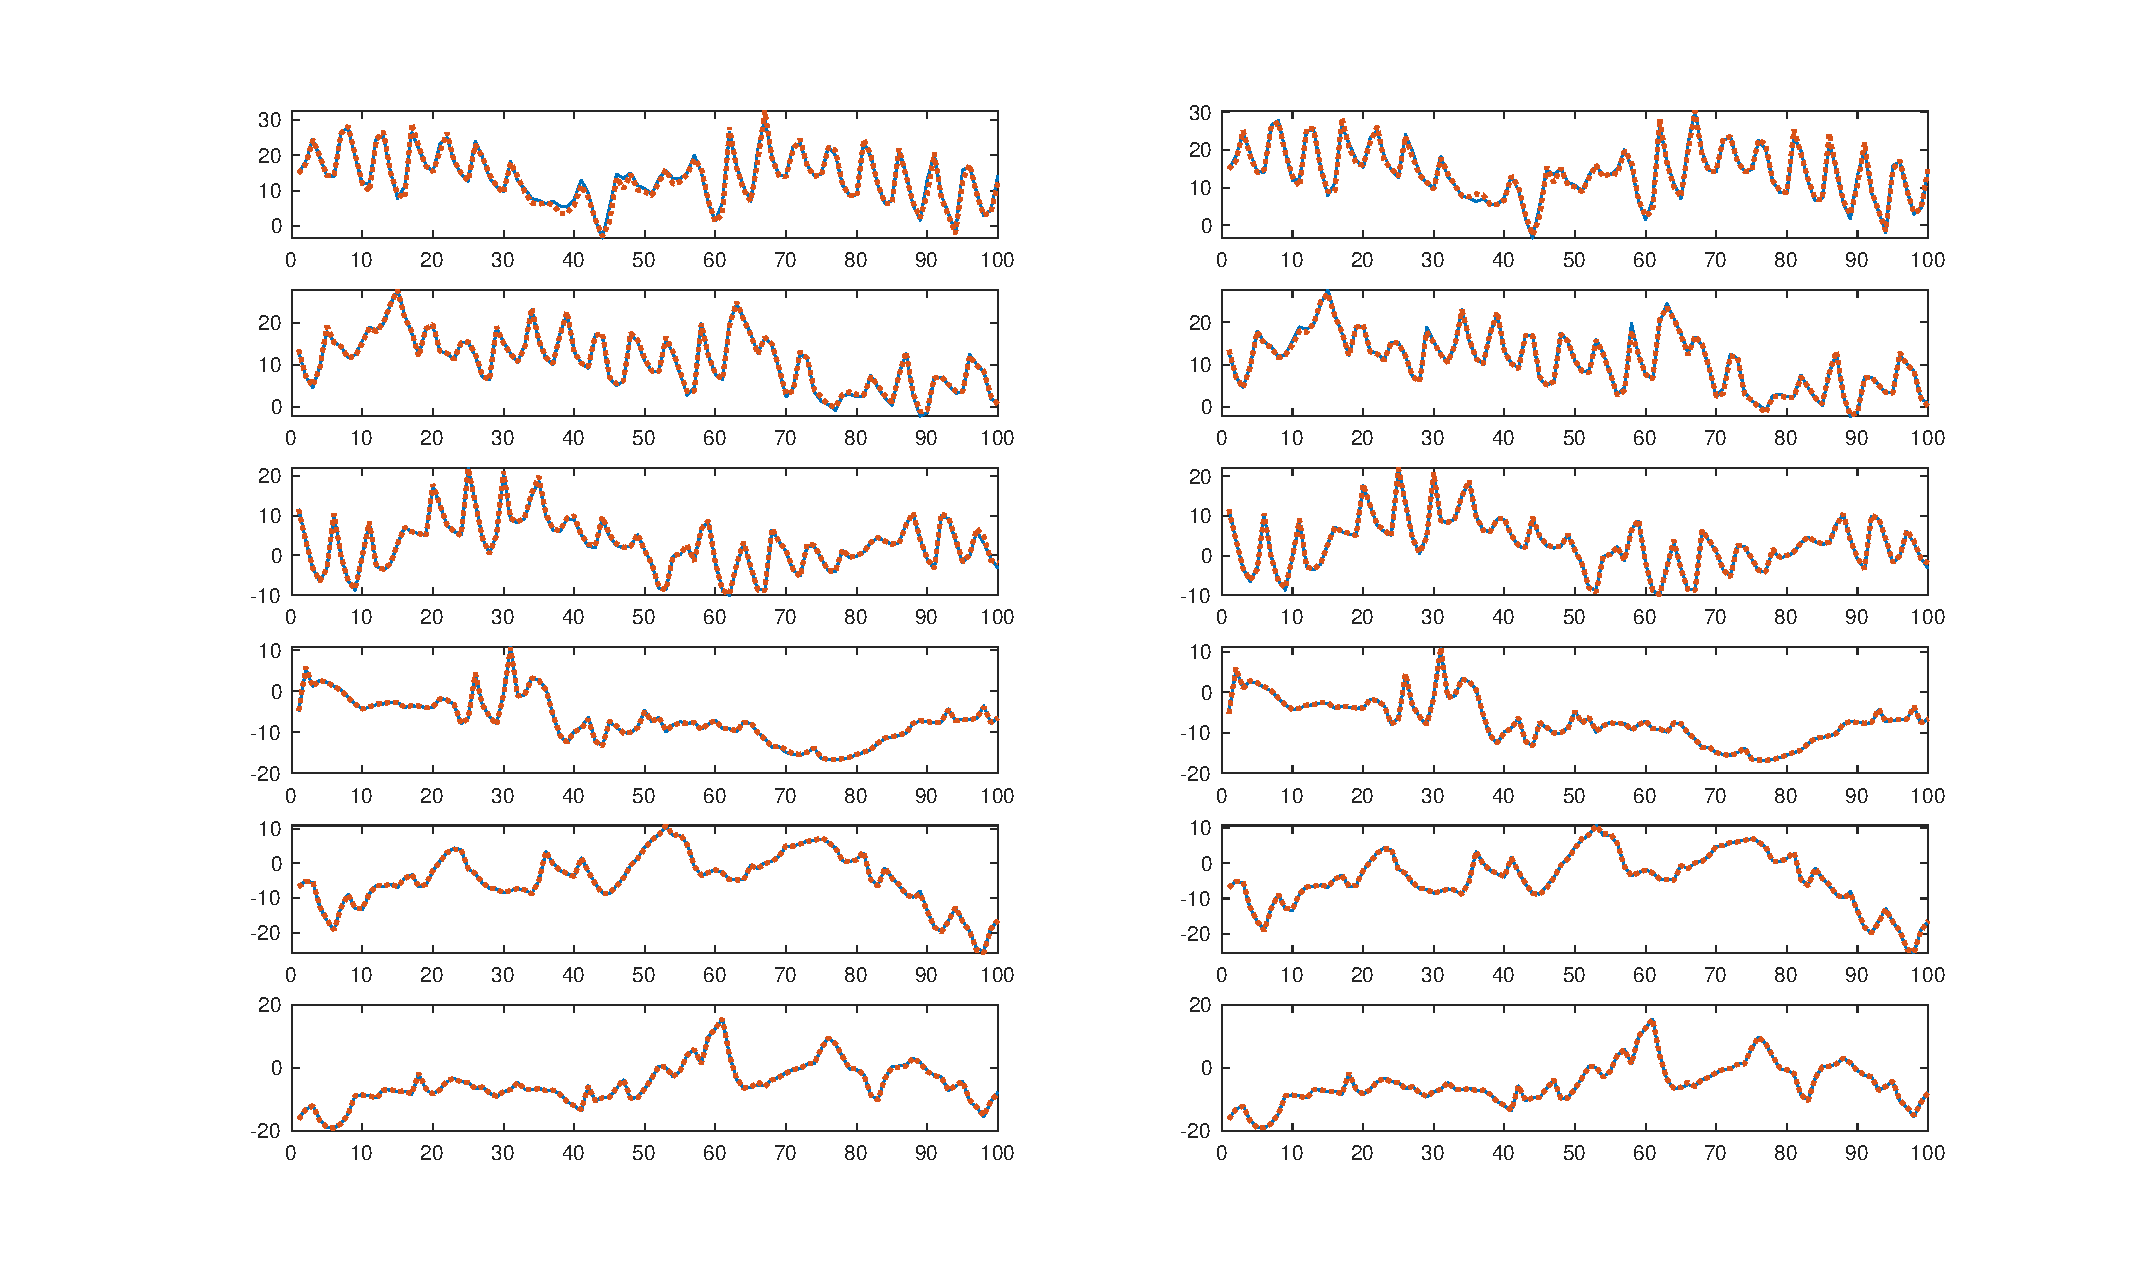
\includegraphics[width=1\columnwidth]{exp/fig_weather.eps}
%	\caption{在耶拿气候预测任务上的系统运行效果,图中左侧为使用采样方法生成简化网络,右侧为使用预存投影矩阵方法生成简化网络,图中自上至下表示的网络阶数分别
%	为10,20,30,40,60,80。实线表示原始网络的模型预测值,虚线表示简化网络的模型预测值。}
%	\label{fig:second}
%\end{figure}
